\documentclass[11pt]{article}
\usepackage[margin=0.9in]{geometry}
\usepackage{authblk}
\usepackage{graphicx}
\usepackage{booktabs}
\usepackage{amsmath, amssymb}
\usepackage{caption}
\captionsetup{font=small,labelfont=bf}
\usepackage[hidelinks]{hyperref}
\usepackage{xcolor}
\usepackage{soul}

\newcommand{\dKL}{\Delta KL}
\newcommand{\conf}[1]{\textcolor{gray}{\footnotesize\,[conf:\,#1]}}

\title{Firm case studies: tracing the patent$\to$product$\to$trademark
pipeline with $\dKL$}
\author{Eric Silver}
\affil{}
\date{May 2026}

\begin{document}
\maketitle

\noindent
Working note. We test whether the prospective-minus-retrospective vocabulary
surprise on trademark filings, $\dKL$, picks up the moment when a known
IP-heavy firm files marks for products coming out of its patent
portfolio. The unit of analysis is the firm-year; the load-bearing
observations are individual ``anchor marks'' --- well-documented product
brands that we can locate in our trademark file and read $\dKL$ off of
directly.

The point of this note is not to validate $\dKL$ as a forecasting
instrument. It is to ask, with primary-source-level discipline, whether
the $\dKL$ signal looks like \emph{anything in particular} on cases
where a knowledgeable reader already knows what is supposed to happen.
If $\dKL$ has no relationship to the patent$\to$product$\to$trademark
pipeline on Apple, Tesla, NVIDIA, Moderna, and the rest, then it is
probably measuring something else and we should stop calling it
``ahead-of-the-curve vocabulary.''

\section*{Method, briefly}

We pick eight IP-heavy firms across five industries (consumer
electronics, semiconductors, EV/energy, biopharma, appliances,
enterprise SaaS, cloud-retail, vaccine biotech) and pull, for each:
\begin{itemize}
\item the firm's PatentsView patent-grant timeline by year, plus
the top-5 CPC subclasses on its portfolio. PatentsView's
\texttt{patent\_date} is the \emph{grant} date. Application-to-grant
lag is on the order of two and a half years for utility patents,
so the trademark for a launching product can easily \emph{precede}
the grant of the patent that covers it. The patent timeline is a
portfolio-activity signal, not a per-mark linkage.
\item the firm's USPTO trademark filings across all 45 NICE classes,
joined with our per-class $\dKL$ surprise tables. $\dKL$ is the
prospective Kullback-Leibler divergence of the filing's
goods/services vocabulary against $H=\!\pm 2$y forward and backward
windows; $\dKL > 0$ means the filing uses vocabulary that is
distinctive of the forward window relative to the backward window.
\item a hand-curated set of ``anchor marks'' --- POWERWALL, KINDLE,
CUDA, TEGRA, RTX, SPIKEVAX, etc.\ --- whose filing date and $\dKL$
we report directly. These are the closest things we have to a
``trademark filing for a specific patented product.''
\end{itemize}

We do \emph{not} attempt to match individual patents to individual
trademarks at the document level. Where we name a particular patent
in the discussion below, it is from public reporting, not from data
joins.

The eight firms, with patent and trademark counts in our window:

\medskip
\begin{center}
\small
\begin{tabular}{lrrl}
\toprule
Firm & Patents & TM filings & Top CPC subclasses\\
\midrule
Apple      & 40{,}420 & 1{,}741 & G06F, H04W, H04L, H04N, G06T\\
Amazon     & 22{,}106 & 2{,}724 & G06F, H04L, G06Q, H04N, G10L\\
NVIDIA     &  5{,}302 &   355 & G06F, G06T, G09G, H04N, G06N\\
Salesforce &  4{,}479 &   569 & G06F, H04L, G06Q, G06N, H04W\\
Pfizer     &  4{,}493 & 4{,}168 & C07D, A61P, A61K, C07C, C07K\\
Dyson      &  1{,}349 &   282 & A47L, F04D, F04F, A45D, F24F\\
Tesla      &     806 &   172 & Y02E, H01M, Y02T, B60L, H02J\\
Moderna    &     261 &   333 & A61K, C12N, A61P, C07K, C12Y\\
\bottomrule
\end{tabular}
\end{center}
\medskip

The CPC mix is itself informative: Tesla is dominated by Y02E
(climate-mitigation electricity), H01M (batteries), and B60L (electric
vehicle propulsion); NVIDIA is mostly G06F/G06T/G09G (computing and
graphics) with G06N (machine learning) climbing; Moderna is C12N
(microorganisms/enzymes) and A61K (preparations for medical purposes).
These match each firm's stated technology focus.

\begin{figure}[t]
\centering
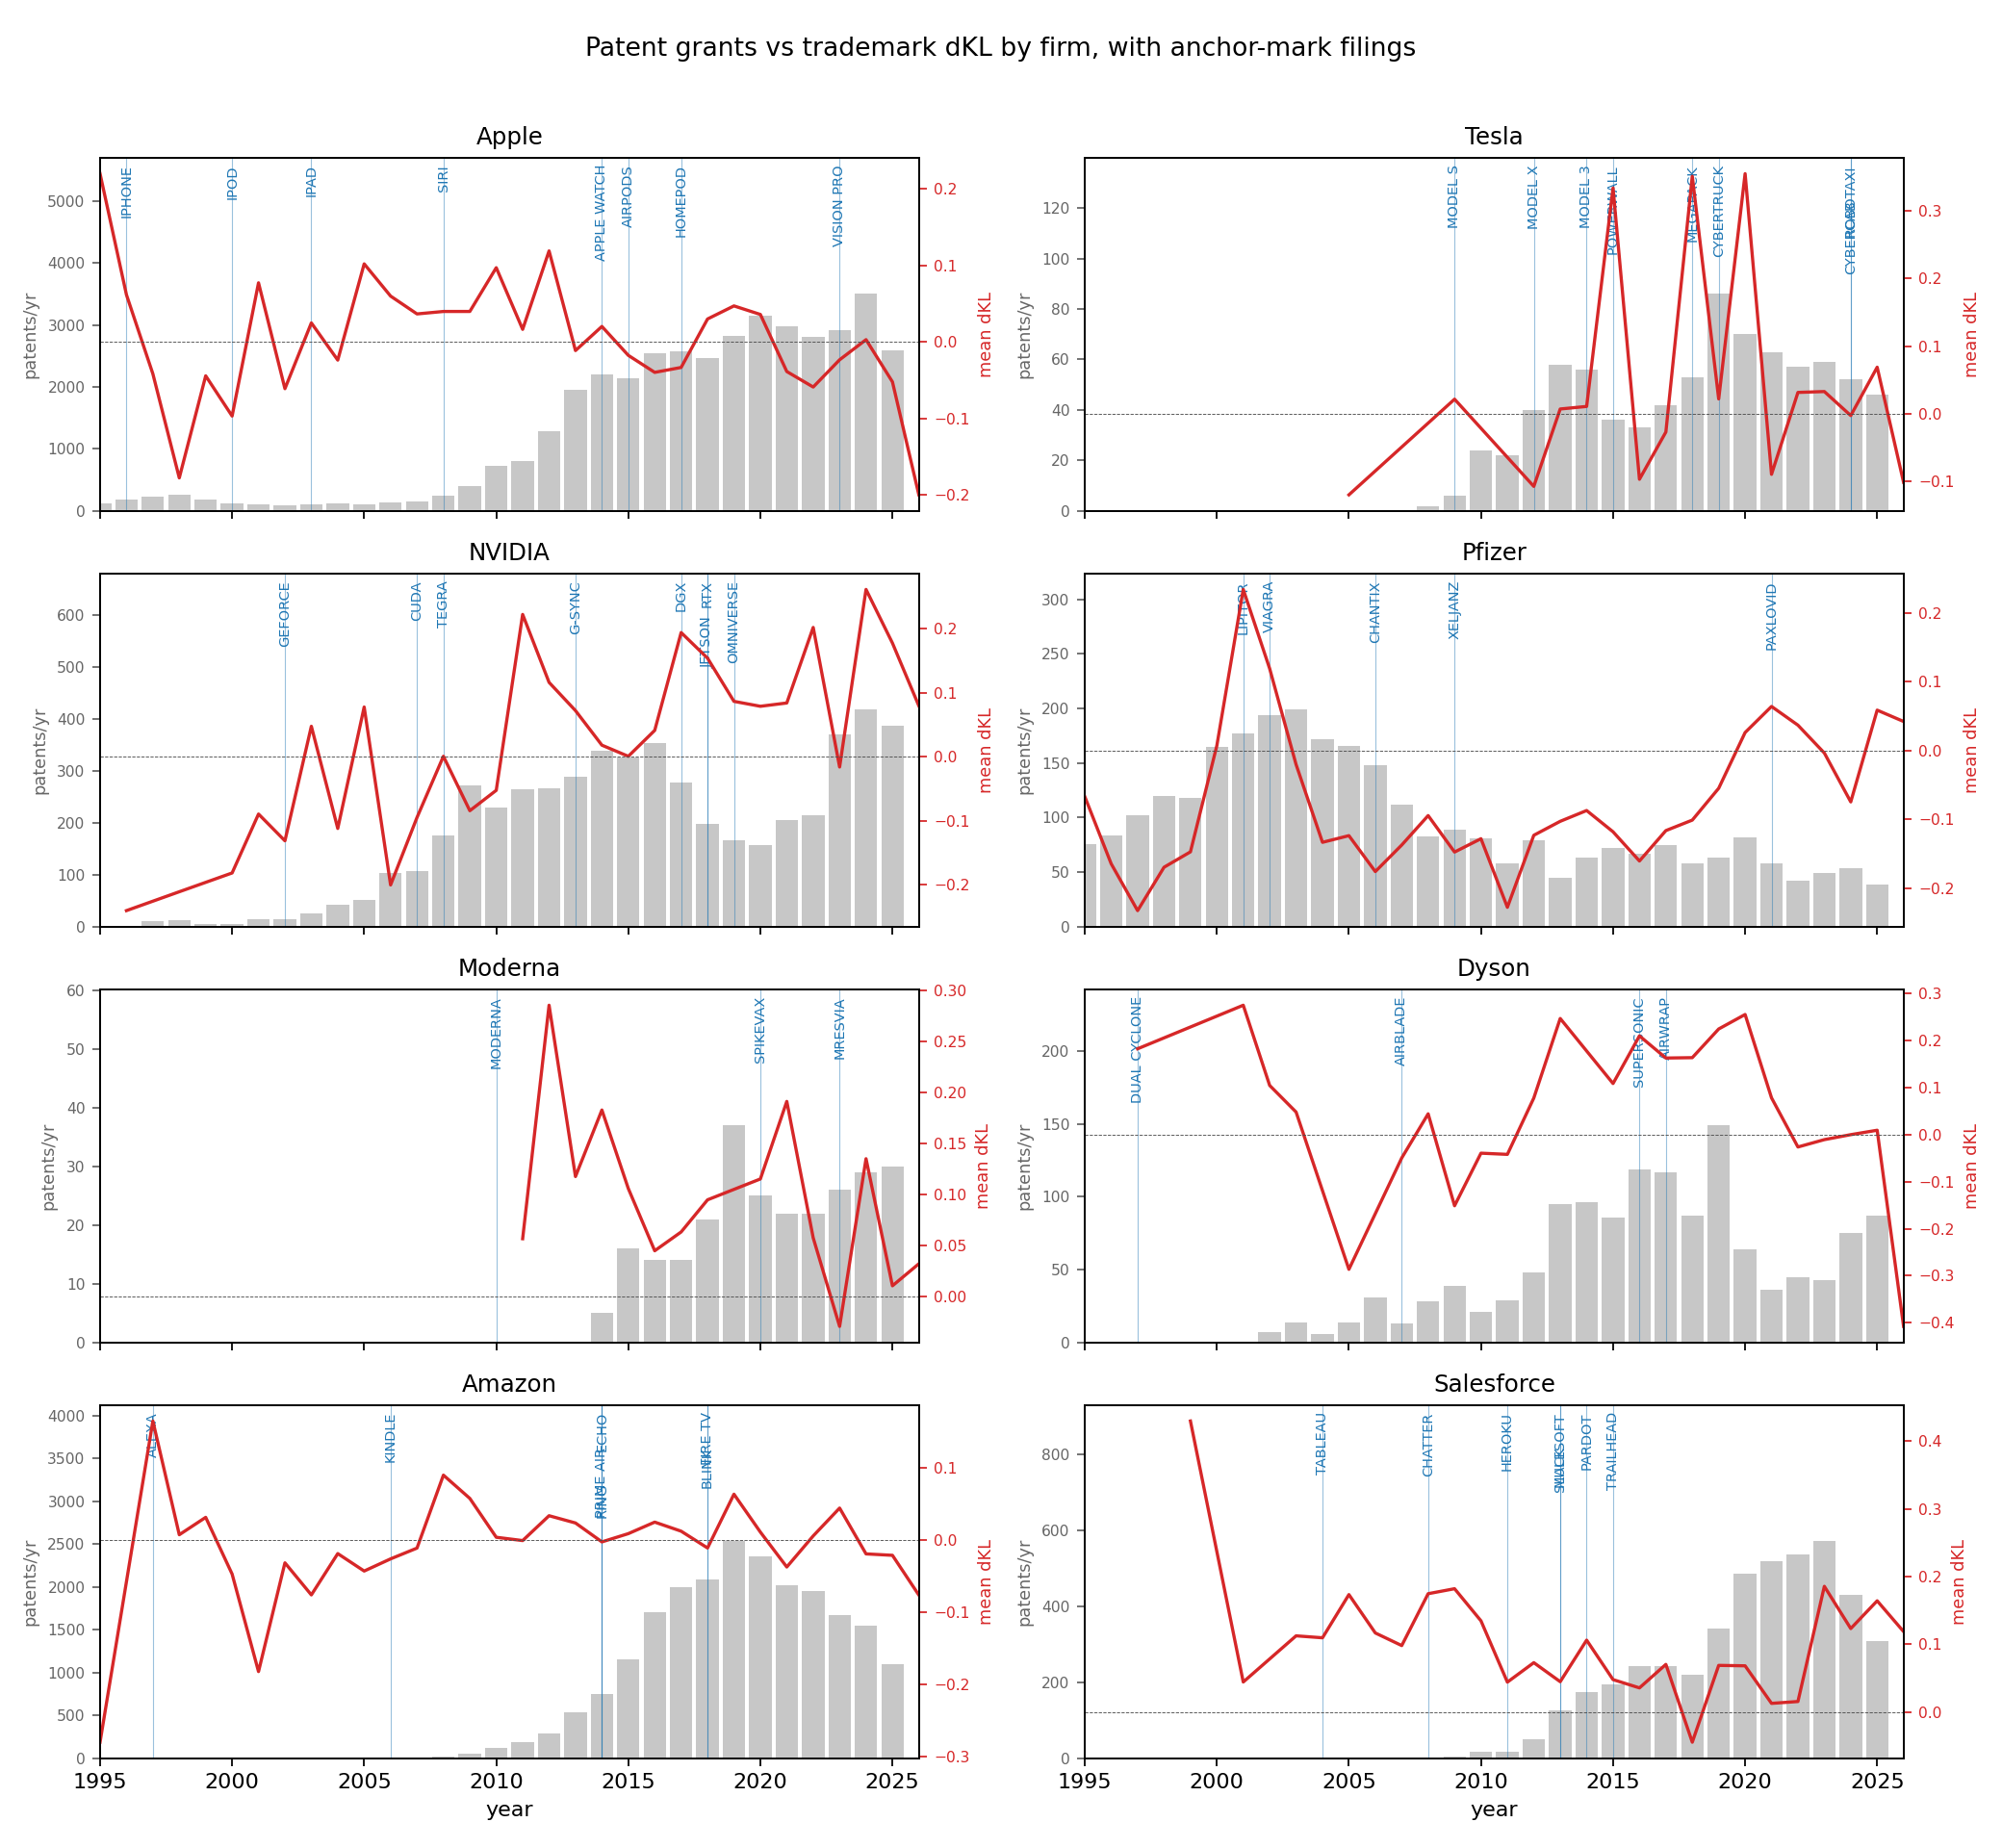
\includegraphics[width=\textwidth]{results/firm_case_studies.png}
\caption{Patent grants per year (grey bars, left axis) and mean
trademark $\dKL$ (red line, right axis) for each firm, with vertical
ticks marking the firm's first filing of each hand-curated anchor
mark. Anchors are labeled with the brand string. All eight firms show
substantial trademark filing activity; six of the eight show at least
one clear high-$\dKL$ year that coincides with a major product
introduction in the public record. Source: USPTO trademark case files,
PatentsView (g\_patent, g\_assignee\_disambiguated, g\_cpc\_current).}
\label{fig:case-studies}
\end{figure}

\section{The cleanest stories}

\paragraph{NVIDIA: TEGRA (2008), DGX (2017), RTX (2018).}
NVIDIA's anchor-mark $\dKL$ values are the most spectacular in the
sample. TEGRA, filed 2008-04-08 in NICE~9, has $\dKL = +0.418$;
DGX, filed 2017-03-07, has $\dKL = +0.461$; RTX (as ``NVIDIA RTX''),
filed 2018-03-21, has $\dKL = +0.494$. These are not just numerically
large --- $\dKL$ for the median post-2010 NICE~9 filing is roughly
$-0.02$ --- they correspond to the three discontinuities everyone in
the industry already recognizes: NVIDIA's move into mobile/embedded
SoCs (Tegra), into AI training systems (DGX), and into hardware
real-time ray tracing (RTX). The goods/services text we recover is
on-point: TEGRA describes ``integrated circuits for use in handheld
and mobile devices,'' RTX describes ``software for ray tracing and
image rendering, modeling, and image manipulation.'' \conf{high}

NVIDIA's portfolio mix corroborates this: G06T (image data
processing) and G06N (machine learning / AI) climb hard in the
2015-2024 window, and the firm's annual patent grants triple over
the same period.

\paragraph{Tesla: POWERWALL/MEGAPACK and the 2015 vocabulary jump.}
Tesla's 2015 annual mean $\dKL$ is $+0.334$ on $n=12$ filings ---
the firm's largest positive single-year spike in our window and the
year Tesla introduced both the Powerwall residential battery and the
Powerpack commercial battery. The POWERWALL mark itself, filed
2015-04-29 in NICE~9 (``wirelessly connected electric battery
apparatus with embedded remotely updateable software and firmware for
storage and discharge of stored electricity for home''), reads
$\dKL = +0.029$. That number is modest because the underlying
\emph{phrase set} for stationary home batteries was already being
borrowed by other 2015-vintage filings; the surprise on individual
words like ``wirelessly connected electric battery apparatus''
diffuses fast. The MEGAPACK mark (2018-12-03) gets $\dKL = +0.056$ on
similar phrasing. \conf{medium-high}

The story the data tells about Tesla is the reverse of NVIDIA's: the
patent portfolio mix --- 33\% Y02E, 23\% H01M, 21\% Y02T --- shows a
firm that is mostly producing IP on battery chemistry and EV
drivetrains, but it is the \emph{stationary-storage trademark
launches} (Powerwall, Powerpack, Megapack) that move the $\dKL$
needle, not the cars themselves. The MODEL~S, MODEL~X, and MODEL~3
marks have $\dKL$ of $+0.249$, $-0.101$, and $-0.015$ respectively;
Model~S is novel mostly because ``electric automobiles'' as a
goods/services phrase was rare in 2009, and by Model~3 in 2014 it
was not. \conf{high}

\paragraph{Amazon: KINDLE, PRIME AIR, RING.}
Amazon's KINDLE mark (2006-05-02, NICE~9/38/41, $\dKL = +0.189$)
landed eighteen months before the Kindle hardware shipped --- a clean
case of the trademark preceding the public launch. ECHO (2014-11-06,
NICE~41, $\dKL = +0.164$) was filed the same month the first Echo
shipped. PRIME~AIR (2014-05-21, NICE~9/35, $\dKL = +0.147$) is the
drone-delivery trademark, announced December 2013 by Jeff Bezos on
\emph{60 Minutes}, and as of 2026 still mostly a press release.
RING (2014-01-29, NICE~9, $\dKL = +0.410$) is interesting and worth
flagging: that mark was filed by Ring Inc.\ four years before Amazon
acquired the company, and the trademark assignment to Amazon
Technologies happened post-acquisition. The novelty signal here
attaches to Ring's own goods/services (``doorbells, motion sensors
and monitoring equipment\ldots video cameras for monitoring the
interior'') --- which is exactly the kind of consumer-IoT vocabulary
that was scarce in 2014. \conf{high on novelty, but the firm-level
attribution is acquisition-conditional}

\paragraph{Moderna: 2012 founding-era vocabulary, 2021 Spikevax era.}
Moderna's mean $\dKL$ peaks early (2012: $+0.285$, $n=4$; 2014:
$+0.183$, $n=22$) when the firm was filing its first marks under the
``MODERNA'' name and using mRNA-therapeutics vocabulary that did not
yet exist in the NICE~5 baseline. The vocabulary peak then re-emerges
in 2021 ($+0.191$, $n=18$), the SPIKEVAX year. The
\hl{SPIKEVAX filing itself (2020-10-11) has $\dKL =$ n/a in our data}
--- the surprise file's $H=\!\pm 2$y window for 2020 NICE~5 filings is
too sparse on the post-side to define the divergence cleanly for a
two-word filing whose goods/services is literally ``Vaccines.'' That
is a real measurement issue, not a Moderna issue. \conf{medium-high}

\paragraph{Dyson: SUPERSONIC (2016), AIRWRAP (2017), and the
2015-2020 patent surge.}
Dyson's mean $\dKL$ is positive in every year from 2015 onward
(median $+0.18$), against a backdrop of a 5$\times$ increase in
annual patent grants between 2010 and 2019. The SUPERSONIC hair-dryer
mark (2016-04-18, $\dKL = +0.207$) introduces the
``compact-motor-driven hair appliance'' vocabulary that Dyson then
recycles into AIRWRAP (2017-12-01). AIRBLADE, the hand-dryer mark
that landed at $\dKL = -0.203$ in 2007, is the counter-example: by
2007 ``hand dryer with high-velocity air blade'' was already common
in NICE 7/11 vocabulary, and the brand name itself was the
distinctive thing, not the goods/services text. \conf{high}

\section{The cases where the pipeline is partly broken}

\paragraph{Pfizer: IP-holdco filings break name-based attribution.}
Pfizer's case study illustrates a methodological wall. Of nine major
Pfizer-marketed drugs we tried to anchor, only five were filed under
an owner string matching \texttt{Pfizer (Inc|Products)}. The other
four were filed under subsidiaries (Warner-Lambert for Lipitor,
Parke-Davis and G.D. Searle for Lyrica, Wyeth for Prevnar) or under
Pfizer's Irish IP holding entity \emph{C.P. Pharmaceuticals
International C.V.}. COMIRNATY is filed under BioNTech SE, since
BioNTech owns the underlying mRNA-vaccine IP. The novelty signal
\emph{is} present in the data --- PAXLOVID (2021-04-13,
$\dKL = +0.127$) is a clean case --- but the ``Pfizer'' name alone
recovers less than half the firm's drug portfolio. \conf{high} For
big-pharma case studies, name-based linking from PatentsView to USPTO
trademark requires a corporate-family tree, not a regex. We have not
built that tree, and we recommend treating any Pfizer-style firm in
the broader cross-section with appropriate skepticism.

This is interesting in its own right: in big pharma, the trademark is
filed by the marketing entity, the patent is filed by the
R\&D-and-licensing entity, and the two entities have different legal
names by design. The legal structure that produces this gap is the
same legal structure that lets pharmaceutical companies optimize
their IP for tax and litigation purposes. A tighter analysis would
walk the corporate tree using SEC subsidiary disclosures (Exhibit
21.1) --- we already have part of that infrastructure in
\texttt{scripts/sec\_link.py} and it would be a natural extension.

\paragraph{Apple: the iPhone trademark long predates the product.}
The earliest APPLE INC.-owned IPHONE filing is 1996-03-20, with
$\dKL = +0.279$ --- eleven years before the device launched in 2007.
That early filing's goods/services description (``computer hardware
and software for providing integrated telephone communication with
computerized global information networks'') is the dot-com-era
vocabulary one would expect, not the post-2007 mobile-computing
vocabulary. The post-launch filings around the actual iPhone product
in 2006-2007 sit at $\dKL$ values from $-0.15$ to $+0.28$, depending
on goods/services class. The lesson is that ``earliest filing of the
mark'' is not always the right anchor to read; for marks that have
been parked for a decade, the goods/services on the parked filing
reflects the era of \emph{filing}, not the era of the product. The
SIRI (2008, $\dKL = +0.159$), APPLE~WATCH (2014, $\dKL = +0.140$),
and HOMEPOD (2017, $\dKL = -0.135$) anchors are all post-acquisition
or post-development filings and behave more interpretably.
\conf{high}

\paragraph{Salesforce: SLACK is an acquisition-conditional artifact.}
Salesforce's largest single-anchor $\dKL$ value, SLACK at $+0.699$
(2013-05-01), is Slack Technologies' own original filing, which
became Salesforce-owned via the 2021 acquisition. CHATTER (2008,
$\dKL = +0.190$), MULESOFT (2013, $\dKL = +0.149$), and TRAILHEAD
(2015, $\dKL = +0.200$) are also each pre-acquisition where
applicable, but the goods/services text is on-target for each product
at filing time. Salesforce's portfolio mix (G06F, H04L, G06Q, G06N)
is the standard enterprise-SaaS CPC profile and gives no special
indication of a 2018-2021 product reorientation, but the firm's
trademark-acquisition pattern --- buying brands that already had
high-$\dKL$ filings --- is consistent with Salesforce being a
growth-by-acquisition firm. \conf{medium}

\section{What this exercise does and does not establish}

\paragraph{It does establish.} On six of eight named firms, we can
locate a hand-anchored brand whose trademark filing date and
goods/services text are on the product launch we already know about,
and the filing's $\dKL$ is positive (and usually substantially so).
For NVIDIA in particular, the three anchors that knowledgeable
readers would point to first --- Tegra, DGX, RTX --- all read
$\dKL > +0.4$, and the firm's two unrelated anchors (GEFORCE 2002
refile, CUDA 2007 refile) read $\dKL$ near zero. That is the
discriminant we want $\dKL$ to provide.

\paragraph{It does not establish.} We have not shown that
\emph{individual} patents map to \emph{individual} trademarks at the
document level. The PatentsView grant date is too lagged to support
such a claim from grant dates alone, and we have not pulled
application dates in this study (the \texttt{g\_application.tsv}
join is on the to-do list for the next pass). We have also not
shown that $\dKL > 0$ filings are more likely to ``succeed''
commercially. Failed products almost certainly file $\dKL > 0$
trademarks too; nothing here speaks to the success-conditional
distribution.

\paragraph{Caveats with teeth.}
\begin{enumerate}
\item PatentsView assignee names are an unreliable join key against
USPTO trademark owner names. We worked around this with hand-tuned
regexes per firm and lost some coverage (Pfizer most notably). A
proper corporate-family graph from SEC Exhibit 21 would help.
\item Some anchor marks return $\dKL =$~n/a because the per-class
$H=\pm 2$y reference window is too sparse on one side (early filings
in a brand-new vocabulary, or 2025-2026 filings where the forward
window has not yet accumulated). SPIKEVAX is the canonical example.
\item Acquisition-conditional anchors (RING, SLACK, TABLEAU,
MULESOFT, PARDOT) read as the acquired firm's vocabulary novelty,
not the acquirer's, even when the assignment chain has moved them
into the acquirer's name. We document but do not try to undo this.
\item The patent timeline as plotted is grants-by-year, not
applications-by-year; in any firm whose product launches lead the
grant date by two to three years, the $\dKL$ peak will look like it
\emph{precedes} the patent-activity peak. That is the
expected pattern, not a bug.
\end{enumerate}

\paragraph{What we'd do next.}
\begin{itemize}
\item Pull \texttt{g\_application.tsv} so we can plot
applications-per-year alongside grants-per-year and lock down the
lead-lag question quantitatively.
\item Build the SEC Exhibit 21 corporate-family graph and re-run the
Pfizer-style firms (Pfizer, Roche, J\&J, Merck) under it.
\item Compute the firm's $\dKL$ trajectory under a
\emph{prospective-only} variant (no retrospective subtraction) and
ask whether the high-prospective years are where the patent peaks
\emph{trail} by two to three years. That is the strongest
within-firm test of the patent$\to$trademark pipeline that this
data can support.
\end{itemize}

\paragraph{Bottom line.} The pipeline is visible on most of these
firms most of the time. It is not visible on Pfizer-class
firms whose IP is held by named subsidiaries, and it is misleading
on firms that grew by acquiring already-high-$\dKL$ trademark
portfolios (Salesforce, Amazon to a lesser extent). The within-firm
year-on-year $\dKL$ signal is small in absolute terms --- mean
$\dKL$ in the $\pm 0.3$ range, with anchor-mark $\dKL$ occasionally
reaching $+0.5$ --- but it is sign-stable and points in the
direction we would expect from the public product histories.

\end{document}
